\chapter{Механизм Хиггса: как калибровочный бозон приобретает массу}

Теперь мы соединяем две идеи, развитые в предыдущей лекции. Комплексное скалярное поле с нарушенной глобальной симметрией \(U(1)\) содержит массивное радиальное колебание и безмассовое угловое колебание. Локально инвариантная теория \(U(1)\) содержит безмассовое калибровочное поле. Когда скалярное поле заряжено и его равновесный модуль ненулевой, эти утверждения нельзя просто сложить вместе. Угловая мода и калибровочное поле объединяются: калибровочное поле становится массивным, кажущийся бозон Голдстоуна перестает быть независимой частицей, а радиальная хиггсовская мода остается.

Фотон послужит нам модельным калибровочным бозоном, но не тем физическим результатом, к которому мы придем. Электромагнитная \(U(1)\) не нарушена в вакууме, поэтому реальный фотон безмассов. Тот же механизм действует на \(W^\pm\) и \(Z\) в электрослабой теории, где калибровочная группа и скалярный мультиплет устроены сложнее. Абелева модель показывает механизм, не скрывая его за групповой теорией.

\begin{classroomqa}\audiencequestion{Означало ли предыдущее обсуждение, что механизм Хиггса сообщает массу реальному фотону?\lecturetimestamp{00:00:23}}\lecturerresponse{Нет. Мы спрашиваем, что произошло бы \emph{если} бы связанная с фотоном симметрия \(U(1)\) находилась в нарушенной фазе. Такой гипотетический фотон стал бы массивным. Реальный электромагнитный вакуум не находится в этой фазе; в физике элементарных частиц речь вместо этого идет о массе \(W\) и \(Z\).}\end{classroomqa}

Симметрия, связанная с сохранением электрического заряда, — это фазовое вращение \begin{equation}
  \phi(x)\longmapsto e^{i\theta}\phi(x),
\end{equation} внутреннее вращение, называемое \(U(1)\). Сверхпроводник дает реальный аналог нарушенной фазы. Внутри него электромагнитное поле имеет конечную глубину проникновения и в важных отношениях ведет себя как массивное поле. Вне него вновь появляется обычный безмассовый фотон.

\section{Что означает масса для поля}

\subsection{Дисперсия и щель при нулевом импульсе}

Прежде чем вводить поле Хиггса, полезно точно определить, что мы понимаем под массой. Для волны \begin{equation}
  E=\hbar\omega,
  \qquad
  p=\hbar k,
  \label{eq:l08-quantum-wave}
\end{equation} поэтому график \((E,p)\) и график \((\omega,k)\) содержат одну и ту же информацию с точностью до множителей \(\hbar\). В пустом пространстве безмассовое релятивистское возбуждение подчиняется \begin{equation}
  E=c|p|,
  \qquad
  \omega=c|k|.
  \label{eq:l08-massless-dispersion}
\end{equation} Два знака \(k\) соответствуют противоположным направлениям распространения. Существенный момент состоит в том, что \(\omega\) стремится к нулю, когда \(k\) стремится к нулю.

Массивная релятивистская частица подчиняется \begin{equation}
  E^2=c^2p^2+m^2c^4.
  \label{eq:l08-massive-dispersion}
\end{equation} В единицах \(c=\hbar=1\) получаем \begin{equation}
  \omega^2=k^2+m^2.
\end{equation} При \(k=0\) энергия равна \(E=mc^2\), или просто \(m\) в естественных единицах. Следовательно, масса — это ненулевая энергетическая щель моды с нулевым импульсом.

\begin{figure}[htbp]\centering
\begin{adjustbox}{max width=\linewidth}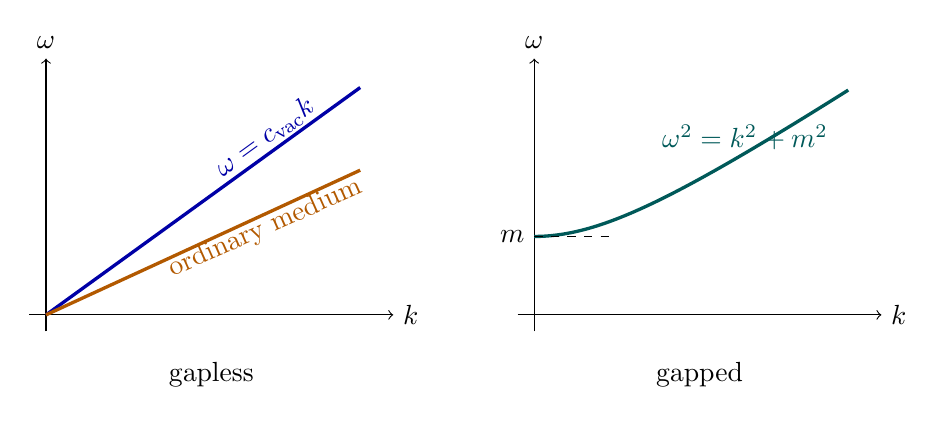
\begin{tikzpicture}[x=1.05cm,y=1.05cm]
  \begin{scope}
    \draw[->] (-0.2,0) -- (4.2,0) node[right] {\(k\)};
    \draw[->] (0,-0.2) -- (0,3.1) node[above] {\(\omega\)};
    \draw[very thick,blue!65!black] (0,0) -- (3.8,2.75);
    \draw[very thick,orange!70!black] (0,0) -- (3.8,1.75);
    \node[blue!65!black,rotate=36] at (2.65,2.15)
      {\(\omega=c_{\rm vac}k\)};
    \node[orange!70!black,rotate=24] at (2.65,1.05)
      {ordinary medium};
    \node[below] at (2,-0.45) {gapless};
  \end{scope}
  \begin{scope}[xshift=6.2cm]
    \draw[->] (-0.2,0) -- (4.2,0) node[right] {\(k\)};
    \draw[->] (0,-0.2) -- (0,3.1) node[above] {\(\omega\)};
    \draw[very thick,domain=0:3.8,samples=120,smooth,teal!70!black]
      plot (\x,{sqrt(0.9+0.45*\x*\x)});
    \draw[dashed] (0,0.95) -- (1.0,0.95);
    \node[left] at (0,0.95) {\(m\)};
    \node[teal!70!black] at (2.55,2.15)
      {\(\omega^2=k^2+m^2\)};
    \node[below] at (2,-0.45) {gapped};
  \end{scope}
\end{tikzpicture}\end{adjustbox}\caption{Изменение скорости распространения меняет наклон бесщелевого дисперсионного соотношения. Придание возбуждению массы открывает ненулевую щель при \(k=0\).}\label{fig:l08-dispersion}\end{figure}

Обычная прозрачная среда может уменьшать фазовую скорость волны, не создавая при этом такой релятивистской массовой щели. На границе частота падающей волны фиксирована, тогда как волновое число подстраивается под дисперсионное соотношение среды. Изменение наклона — не то же самое, что смещение вверх точки пересечения с осью ординат. \editorialnote{Среда может иметь несколько электромагнитных ветвей, а плазма или резонансная среда могут обладать ненулевой плазменной частотной щелью. В лекции сравнение проводится именно между обычной преломляющей ветвью и сверхпроводящим откликом. В более общем смысле бесщелевость означает \(\omega(k)\to0\) при \(k\to0\); точная линейность требуется не во всякой нерелятивистской среде.}

\begin{classroomqa}\audiencequestion{Приобретает ли фотон массу всякий раз, когда проходит через вещество, например через призму?\lecturetimestamp{00:03:02}}\lecturerresponse{Нет. Преломление может изменить связь между частотой и волновым числом, а значит и скорость распространения, при этом ветвь по-прежнему проходит через \(\omega=0\) при \(k=0\). Сверхпроводящая фаза, напротив, придает электромагнитному отклику конечную обратную длину проникновения, аналог массы.}\end{classroomqa}

\begin{classroomqa}\audiencequestion{Если свет фиксированной частоты входит в стекло, меняется ли именно волновое число?\lecturetimestamp{00:09:20}}\lecturerresponse{Да. Инвариантность относительно сдвигов по времени на стационарной границе сохраняет частоту фиксированной. Поскольку дисперсионная кривая в стекле имеет другой наклон, одному и тому же \(\omega\) соответствует другое \(k\) и, следовательно, другая длина волны.}\end{classroomqa}

Наклон \begin{equation}
  v_g=\frac{d\omega}{dk}
\end{equation} есть групповая скорость волнового пакета. Если этот наклон зависит от \(k\), разные фурье-компоненты движутся с разными скоростями, и пакет расплывается. Поэтому зависимость \(\omega(k)\) называется \emph{дисперсионным соотношением}.

\begin{classroomqa}\audiencequestion{Как называется эта кривая и что означает ее наклон?\lecturetimestamp{00:11:02}}\lecturerresponse{Эта кривая — дисперсионное соотношение. Ее производная \(d\omega/dk\) есть групповая скорость. Постоянный наклон дает одну и ту же скорость всем длинам волн; меняющийся наклон заставляет волновой пакет расплываться. Для нашей цели решающее различие состоит в том, достигает ли кривая начала координат или имеет щель.}\end{classroomqa}

\subsection{Однородное колебание — это частица в покое}

Мода \(k=0\) имеет бесконечную длину волны: поле смещено на одну и ту же величину всюду. Отпустим такое однородное смещение. Если поле колеблется с ненулевой частотой, соответствующий квант имеет ненулевую энергию покоя и является массивным. Если в этом направлении нет восстанавливающей силы, частота обращается в нуль, и мода безмассовая.

Это утверждение классическое. Оно не требует, чтобы пространственно разделенные частицы находились в квантовой суперпозиции. Однородная конфигурация классического поля — это просто одно и то же значение поля, повторяющееся по всему пространству.

\begin{classroomqa}\audiencequestion{Если все поле сдвигается целиком, то это то же самое, что квантовая запутанность?\lecturetimestamp{00:10:04}}\lecturerresponse{Нет. Однородное классическое поле — это одна классическая конфигурация. Запутанность коррелирует различные квантовые альтернативы, например конфигурации спинов вверх--вниз и вниз--вверх. Задание одного и того же значения поля во многих точках само по себе не является запутанностью и не подразумевает мгновенного причинного отклика.}\end{classroomqa}

Для канонически нормированного действительного поля \begin{equation}
  \mathcal L
  =\frac12\partial_\mu\varphi\,\partial^\mu\varphi-V(\varphi),
\end{equation} разложим около равновесного значения \(\varphi_0\): \begin{equation}
  V(\varphi_0+\eta)
  =V(\varphi_0)
   +\frac12V''(\varphi_0)\eta^2+\cdots.
\end{equation} Линейный член в минимуме исчезает, и уравнение поля дает \begin{equation}
  \omega^2=\bm{k}^2+m^2,
  \qquad
  m^2=V''(\varphi_0).
  \label{eq:l08-curvature-mass}
\end{equation} Следовательно, масса — это кривизна потенциала в направлении движения. Плоское направление имеет нулевую кривизну и дает безмассовую моду.

\section{Комплексное скалярное поле с нарушенной симметрией}

\subsection{Радиальное и угловое движение}

Запишем комплексное скалярное поле в декартовых и полярных координатах: \begin{equation}
  \phi=\phi_R+i\phi_I=\rho e^{i\alpha},
  \qquad
  \phi^*=\phi_R-i\phi_I=\rho e^{-i\alpha}.
  \label{eq:l08-polar-field}
\end{equation} Комплексная плоскость — это \emph{внутреннее} пространство поля. В каждой физической точке пространства-времени \(x\) пара \((\phi_R(x),\phi_I(x))\) задает одну точку на этой внутренней плоскости. Ни одна из внутренних осей не является направлением в лаборатории.

\begin{figure}[htbp]\centering
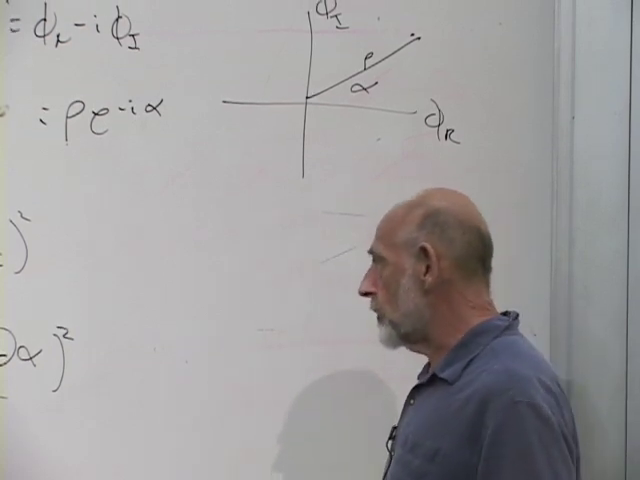
\includegraphics[width=0.72\textwidth]{lecture_08_figure_02.png}\caption{Комплексное скалярное поле, представленное на своей внутренней плоскости \((\phi_R,\phi_I)\). Радиус равен \(\rho\), а \(\alpha\) — внутренняя фаза.}\lectureframe{00:24:41}\label{fig:l08-internal-plane}\end{figure}

Кинетический член скалярного поля принимает вид \begin{align}
  \partial_\mu\phi^*\,\partial^\mu\phi
  &=
  \partial_\mu\phi_R\,\partial^\mu\phi_R
  +\partial_\mu\phi_I\,\partial^\mu\phi_I
  \notag\\
  &=
  \partial_\mu\rho\,\partial^\mu\rho
  +\rho^2\partial_\mu\alpha\,\partial^\mu\alpha.
  \label{eq:l08-polar-kinetic}
\end{align} Глобально \(U(1)\)-инвариантный потенциал зависит от \(\phi^*\phi=\rho^2\), а не от \(\alpha\). Например, \begin{equation}
  V(\phi)
  =\lambda\left(\phi^*\phi-\frac{f^2}{2}\right)^2,
  \qquad \lambda>0.
  \label{eq:l08-mexican-hat}
\end{equation} Его минимумы образуют окружность. Закон инвариантен относительно общего фазового поворота, но выбор одной равновесной фазы выделяет одну точку на окружности.

\begin{figure}[htbp]\centering
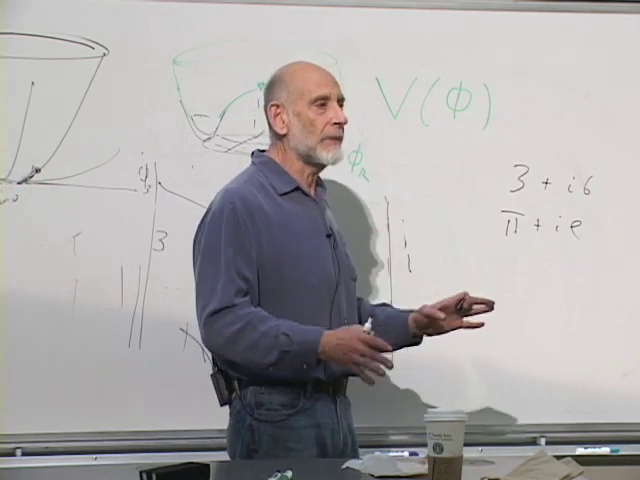
\includegraphics[width=0.78\textwidth]{lecture_08_figure_03.png}\caption{Наброски радиального потенциала на доске. Потенциал симметричен относительно вращений значения поля во внутреннем пространстве, хотя самому полю не обязательно находиться в начале координат.}\lectureframe{00:34:22}\label{fig:l08-radial-potential-board}\end{figure}

\begin{figure}[htbp]\centering
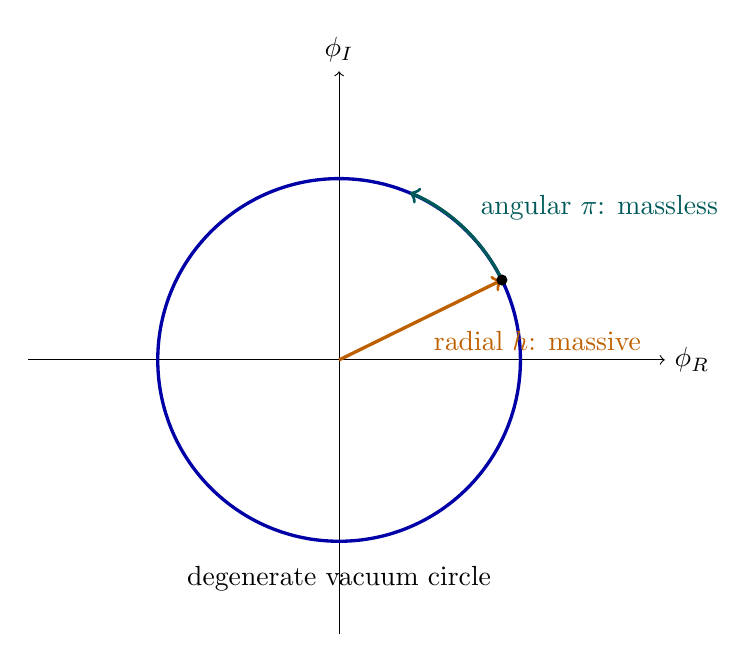
\begin{tikzpicture}[x=0.94cm,y=0.94cm]
  \draw[->] (-4.2,0) -- (4.4,0) node[right] {\(\phi_R\)};
  \draw[->] (0,-3.7) -- (0,3.9) node[above] {\(\phi_I\)};
  \draw[very thick,blue!65!black] (0,0) circle (2.45);
  \draw[->,very thick,orange!75!black] (0,0) -- (2.2,1.08);
  \draw[->,very thick,teal!70!black]
    (2.2,1.08) arc[start angle=26,end angle=67,radius=2.45];
  \node[orange!75!black,below right] at (1.15,0.52)
    {radial \(h\): massive};
  \node[teal!70!black,above right] at (1.78,1.76)
    {angular \(\pi\): massless};
  \fill (2.2,1.08) circle (2pt);
  \node[below] at (0,-2.65) {degenerate vacuum circle};
\end{tikzpicture}\caption{В глобальной теории с нарушенной симметрией есть кривизна по нормали к вакуумной окружности, но нет кривизны вдоль нее. Радиальная хиггсовская мода массивна; угловая голдстоуновская мода безмассовая.}\label{fig:l08-radial-angular}\end{figure}

Положим \begin{equation}
  \phi(x)=\frac{f+h(x)}{\sqrt2}
           e^{i\pi(x)/f}.
  \label{eq:l08-canonical-polar}
\end{equation} Вблизи выбранного вакуума \(h\) описывает радиальное смещение, а \(\pi\) — тангенциальное смещение с каноническими размерностями. Подстановка в ур.~\eqref{eq:l08-polar-kinetic} дает \begin{equation}
  \partial_\mu\phi^*\,\partial^\mu\phi
  =
  \frac12(\partial_\mu h)^2
  +\frac12\left(1+\frac{h}{f}\right)^2
            (\partial_\mu\pi)^2.
  \label{eq:l08-global-expanded}
\end{equation} Потенциал в ур.~\eqref{eq:l08-mexican-hat} дает \begin{equation}
  m_h^2=2\lambda f^2,
  \qquad
  m_\pi^2=0.
  \label{eq:l08-global-masses}
\end{equation} При энергиях, много меньших, чем \(m_h\), радиальное движение требует больших затрат энергии, поэтому можно временно зафиксировать \(h=0\). Оставшийся лагранжиан содержит только \(\frac12(\partial\pi)^2\), без члена \(\pi^2\). Это и есть бозон Голдстоуна.\editorialnote{В двух местах устное объяснение меняет названия местами и говорит, что поглощение голдстоуновской моды сообщает массу бозону Хиггса. Вычисление на доске и оставшаяся часть лекции устанавливают задуманный результат: радиальная кривизна уже придает хиггсовской моде массу, тогда как калибровочный бозон поглощает голдстоуновскую моду и становится массивным.}

\begin{classroomqa}
\audiencequestion{Является ли это единственным спонтанным нарушением симметрии в Стандартной модели?\lecturetimestamp{00:16:39}}
\lecturerresponse{Электрослабая фаза Хиггса — это установленный механизм нарушения симметрии, относящийся к рассматриваемому здесь случаю. Ее фактическая симметрия — \(SU(2)_L\times U(1)_Y\), а не одно лишь \(U(1)\), и в КХД имеется дополнительная вакуумная структура, такая как нарушение киральной симметрии. Абелев пример — это намеренно редуцированная модель механизма калибровочных бозонов.}
\end{classroomqa}

\begin{classroomqa}
\audiencequestion{Придает ли Хиггс массу каждой частице, включая самого себя?\lecturetimestamp{00:17:11}}
\lecturerresponse{Здесь ответ и да, и нет. Электрослабая симметрия запрещает затравочные массы для \(W\), \(Z\) и фермионов Стандартной модели; их массы появляются после того, как поле Хиггса приобретает ненулевую равновесную величину. Масса радиальной моды Хиггса возникает из кривизны его собственного потенциала. Другие гипотетические частицы могут обладать допускаемыми симметрией массами, не связанными с этим механизмом.}
\end{classroomqa}

В лекции такие допускаемые симметрией массы связываются с потенциально очень тяжелыми, трудно наблюдаемыми частицами, и в качестве возможного примера упоминается темная материя. Это мотивация, а не предсказание массы.
\editorialnote{Масштаб массы темной материи остается неизвестным. Предположение в лекции о частице с массой порядка тысячи протонных масс — это историческая спекуляция, а не экспериментально установленное свойство темной материи.}

\begin{classroomqa}
\audiencequestion{Является ли \(\rho\) физическим радиусом, или это значение поля? Что именно радиально симметрично?\lecturetimestamp{00:33:08}}
\lecturerresponse{В каждой точке пространства-времени значение поля представляет собой точку на вспомогательной комплексной плоскости, а \(\rho=|\phi|\) есть расстояние этой точки от начала координат. \emph{потенциал} радиально симметричен на этой внутренней плоскости: все точки с одним и тем же \(\rho\) имеют одну и ту же потенциальную энергию. Этот радиус не является расстоянием в обычном пространстве.}
\end{classroomqa}

\begin{classroomqa}
\audiencequestion{Может ли достаточно сильный радиальный толчок перенести поле через центральный максимум на другую сторону потенциала?
\lecturetimestamp{00:36:00}}
\lecturerresponse{В принципе локальная конфигурация с достаточной энергией может пересечь барьер. Чтобы перевести через него однородное макроскопическое поле, потребовалась бы огромная энергия, а при типичном сильном возмущении энергия ушла бы во множество мод поля, а не была бы когерентно доставлена в противоположную точку. В низкоэнергетическом приближении \(\rho\) фиксируется именно потому, что такие радиальные отклонения там недоступны.}
\end{classroomqa}

\section{Почему комплексная плоскость — не пространство-время}

Различие между физическими и внутренними координатами заслуживает той подробной остановки, которую делает лекция. Скалярное поле называется скалярным, потому что оно инвариантно относительно поворотов физических координатных осей. Два вещественных скалярных поля \(\phi_R(x)\) и \(\phi_I(x)\) при таких поворотах остаются двумя скалярами. Мы можем объединить их в одно комплексное число, но такой способ записи не превращает их в компоненты пространственного вектора.

Глобальное преобразование \(U(1)\) поворачивает \emph{значения} поля:
\begin{equation}
\begin{aligned}
  \phi(x)&\longmapsto e^{i\theta}\phi(x),
  \\
  \rho(x)&\longmapsto\rho(x),
  \\
  \alpha(x)&\longmapsto\alpha(x)+\theta.
\end{aligned}
  \label{eq:l08-global-shift}
\end{equation}
Одна и та же постоянная \(\theta\) используется в каждой точке пространства-времени. Следовательно, \(\partial_\mu\alpha\) не меняется. Это симметрия и потенциала, и обычного кинетического члена. Как только \(\theta\) разрешается зависеть от \(x\), производная обнаруживает это изменение, и рассуждение меняется.

\section{Локализация фазового поворота}

\subsection{Обычная производная не подходит}

Пусть
\begin{equation}
  \phi'(x)=e^{i\theta(x)}\phi(x).
  \label{eq:l08-local-phase}
\end{equation}
Тогда
\begin{equation}
  \partial_\mu\phi'
  =e^{i\theta}
    \left(\partial_\mu\phi+i\,\partial_\mu\theta\,\phi\right).
  \label{eq:l08-ordinary-derivative-fails}
\end{equation}
Лишний член, пропорциональный \(\partial_\mu\theta\), мешает \(\partial_\mu\phi\) преобразовываться так же, как \(\phi\). Следовательно, \(\partial_\mu\phi^*\partial^\mu\phi\) не инвариантно относительно произвольных локальных фазовых поворотов.

\begin{figure}[htbp]
\centering
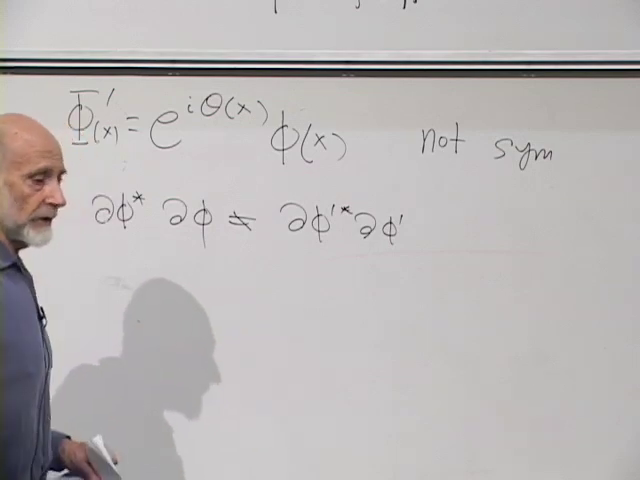
\includegraphics[width=0.78\textwidth]{lecture_08_figure_04.png}
\caption{На доске записаны локальное фазовое преобразование и то, что член с обычной производной не остается инвариантным.}
\lectureframe{00:46:49}
\label{fig:l08-local-not-symmetry}
\end{figure}

Введем векторный потенциал и последовательно зафиксируем одну конвенцию:
\begin{equation}
  D_\mu=\partial_\mu+i g A_\mu,
  \qquad
  A_\mu'=A_\mu-\frac1g\partial_\mu\theta.
  \label{eq:l08-covariant-convention}
\end{equation}
Тогда
\begin{align}
  D_\mu'\phi'
  &=
  \left(\partial_\mu+i g A_\mu'\right)
  e^{i\theta}\phi
  \notag\\
  &=
  e^{i\theta}
  \left[
    \partial_\mu\phi+i(\partial_\mu\theta)\phi
    +i g A_\mu\phi-i(\partial_\mu\theta)\phi
  \right]
  \notag\\
  &=e^{i\theta}D_\mu\phi.
  \label{eq:l08-covariant-transform}
\end{align}
Нежелательные члены сокращаются. Комплексно-сопряженная производная имеет вид
\begin{equation}
  (D_\mu\phi)^*
  =(\partial_\mu-i g A_\mu)\phi^*,
\end{equation}
и ее противоположная фаза сокращается в произведении
\begin{equation}
  (D_\mu\phi)^*D^\mu\phi.
\end{equation}

\begin{classroomqa}
\audiencequestion{Было ли преобразование калибровочного поля в предыдущей лекции записано с противоположным знаком?\lecturetimestamp{00:48:04}}
\lecturerresponse{Одновременная смена знака в \(D_\mu\) и в законе преобразования — всего лишь конвенция. При
\(D_\mu=\partial_\mu+i gA_\mu\) и
\(\phi'=e^{i\theta}\phi\) согласованность требует
\(A_\mu'=A_\mu-g^{-1}\partial_\mu\theta\). Альтернативная конвенция работает столь же хорошо, если одновременно изменить все знаки.}
\end{classroomqa}

\begin{classroomqa}
\audiencequestion{Означает ли использование на доске прописной или строчной формы \(\phi\) другое поле?\lecturetimestamp{00:55:02}}
\lecturerresponse{Никакого различия не имеется в виду. Меняющаяся форма буквы — это почерк, а не дополнительная операция и не второе скалярное поле. Существенные различия задают штрих, звездочка комплексного сопряжения и пространственно-временной индекс.}
\end{classroomqa}

\begin{classroomqa}
\audiencequestion{Является ли комплексное сопряжение той же операцией, что и поднятие или опускание лоренцева индекса в кинетическом члене?
\lecturetimestamp{00:56:50}}
\lecturerresponse{Нет. Звездочка выполняет комплексное сопряжение внутреннего комплексного поля. Лоренцевы индексы поднимаются с помощью метрики пространства-времени:
\(D^\mu=g^{\mu\nu}D_\nu\). Лоренцев скаляр требует свертки \((D_\mu\phi)^*D^\mu\phi\); обе операции здесь присутствуют и служат разным целям.}
\end{classroomqa}

\subsection{Калибровочное поле имеет собственную динамику}

Тензор напряженности поля
\begin{equation}
  F_{\mu\nu}=\partial_\mu A_\nu-\partial_\nu A_\mu
  \label{eq:l08-field-strength}
\end{equation}
калибровочно инвариантен, потому что две смешанные вторые производные от \(\theta\) сокращаются. Его компоненты время--пространство содержат электрическое поле, а компоненты пространство--пространство содержат магнитное поле. Поэтому скалярная версия электродинамики имеет вид
\begin{equation}
  \mathcal L
  =(D_\mu\phi)^*D^\mu\phi
  -V(\phi^*\phi)
  -\frac14F_{\mu\nu}F^{\mu\nu}.
  \label{eq:l08-abelian-higgs}
\end{equation}
Заряженное поле здесь бозонное. Это не электронное поле, которое является фермионным. Заряженное ядро гелия или конденсат куперовских пар показывают, как может возникнуть бозонная заряженная степень свободы.

До нарушения симметрии калибровочный член содержит производные от \(A_\mu\), но не содержит прямого массового члена. Можно было бы попытаться добавить
\begin{equation}
  \frac12m_A^2A_\mu A^\mu,
\end{equation}
но при преобразовании по уравнению~\eqref{eq:l08-covariant-convention}
\begin{equation}
  A_\mu A^\mu
  \longmapsto
  \left(A_\mu-\frac1g\partial_\mu\theta\right)
  \left(A^\mu-\frac1g\partial^\mu\theta\right),
  \label{eq:l08-bare-mass-fails}
\end{equation}
что не равно \(A_\mu A^\mu\). Затравочная масса калибровочного бозона запрещена локальной симметрией.

\begin{figure}[htbp]
\centering
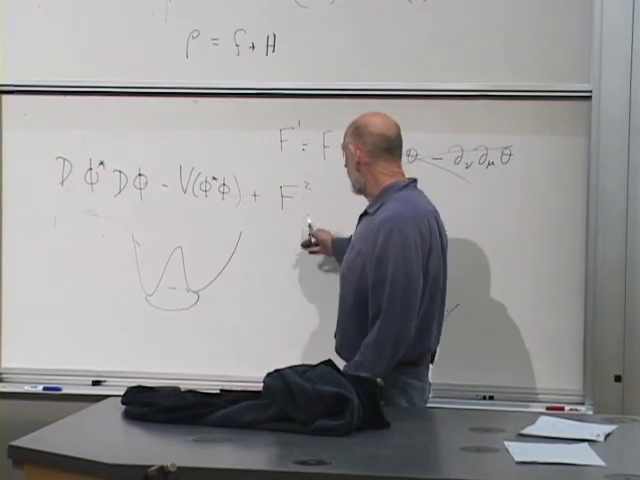
\includegraphics[width=0.76\textwidth]{lecture_08_figure_05.png}
\caption{Проверенное состояние доски для этого препятствия: при калибровочном преобразовании \(A_\mu A^\mu\) превращается в квадрат, содержащий \(\partial_\mu\theta\), так что затравочная масса векторного поля не инвариантна.}
\lectureframe{01:07:30}
\label{fig:l08-bare-mass-board}
\end{figure}

\section{Механизм Хиггса}

\subsection{Ковариантная производная порождает массу}

Вернемся к потенциалу с нарушенной симметрией и используем канонически нормированную параметризацию
\begin{equation}
  \phi(x)=\frac{f+h(x)}{\sqrt2}
  e^{i\pi(x)/f}.
\end{equation}
Ее ковариантная производная равна
\begin{equation}
  D_\mu\phi
  =
  \frac{e^{i\pi/f}}{\sqrt2}
  \left[
    \partial_\mu h
    +i(f+h)
      \left(\frac{\partial_\mu\pi}{f}+gA_\mu\right)
  \right].
  \label{eq:l08-covariant-polar}
\end{equation}
Следовательно,
\begin{equation}
\begin{aligned}
  (D_\mu\phi)^*D^\mu\phi
  ={}&
  \frac12(\partial_\mu h)^2
  \\
  &+\frac12(f+h)^2
    \left(\frac{\partial_\mu\pi}{f}+gA_\mu\right)
  \\
  &\hspace{4.2em}\times
    \left(\frac{\partial^\mu\pi}{f}+gA^\mu\right).
\end{aligned}
  \label{eq:l08-higgs-kinetic}
\end{equation}

Решающему члену не требуется никакой выбор калибровки:
\begin{equation}
  \frac12g^2f^2 A_\mu A^\mu.
  \label{eq:l08-vector-mass-term}
\end{equation}
Сравнивая его с формой Прока
\(\frac12m_A^2A_\mu A^\mu\), получаем
\begin{equation}
  \boxed{m_A=g f}.
  \label{eq:l08-vector-mass}
\end{equation}
То же разложение порождает и взаимодействия
\(g^2fh A_\mu A^\mu\) и
\(\frac12g^2h^2A_\mu A^\mu\). Следовательно, масса вектора не является произвольным нарушением калибровочной симметрии. Она возникает из калибровочно-инвариантного скалярного кинетического члена, вычисленного в фазе с ненулевой равновесной величиной \(f\).

\begin{figure}[htbp]
\centering
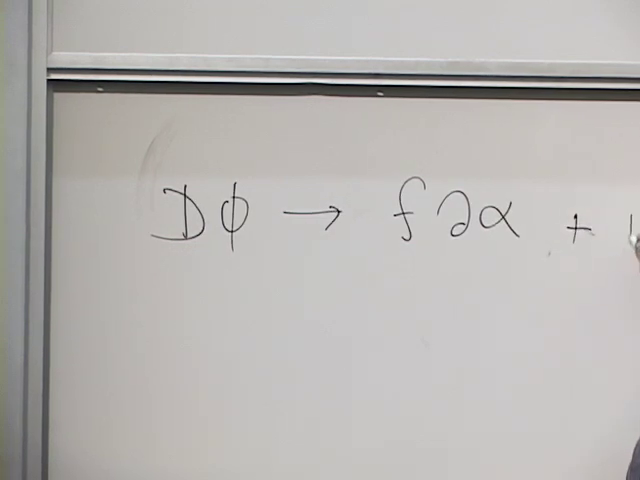
\includegraphics[width=0.78\textwidth]{lecture_08_figure_06.png}
\caption{На доске выделен вклад \(f^2A^2\) внутри \((D\phi)^*(D\phi)\). Численные множители зависят от того, как нормированы скалярное поле и калибровочная константа связи; при уравнениях~\eqref{eq:l08-canonical-polar}
и \eqref{eq:l08-covariant-convention} получается \(m_A=gf\).}
\lectureframe{01:10:10}
\label{fig:l08-generated-mass-board}
\end{figure}

В лекции \(g\) и несколько множителей \(\sqrt2\) поглощаются обозначениями на доске, поэтому при выделении массы там ненадолго чередуются \(f\), \(2f\) и \(\sqrt2f\). Эти множители не имеют инвариантного смысла, пока не заданы нормировки кинетического члена и потенциала. Устойчивый результат — \(m_A\propto gf\); уравнение~\eqref{eq:l08-vector-mass} дает множитель для используемой здесь конвенции.

\subsection{Фаза поглощается}

При калибровочном преобразовании фазовая переменная меняется как
\begin{equation}
  \pi'(x)=\pi(x)+f\,\theta(x).
\end{equation}
Выберем
\begin{equation}
  \theta(x)=-\frac{\pi(x)}{f}.
  \label{eq:l08-unitary-gauge-choice}
\end{equation}
Тогда \(\pi'=0\). Это унитарная калибровка, в которой
\begin{equation}
  \phi'(x)=\frac{f+h(x)}{\sqrt2}
\end{equation}
вещественно, и уравнение~\eqref{eq:l08-higgs-kinetic} сводится к
\begin{equation}
  (D_\mu\phi')^*D^\mu\phi'
  =
  \frac12(\partial_\mu h)^2
  +\frac12g^2(f+h)^2A_\mu'A^{\prime\mu}.
  \label{eq:l08-unitary-gauge-lagrangian}
\end{equation}
Угловое голдстоуновское поле исчезло из списка независимых переменных, а масса вектора сохраняется.

Сначала лекция показывает это в низкоэнергетическом пределе \(\rho=f\), где
\begin{align}
  \phi&=f e^{i\alpha},
  \notag\\
  D_\mu\phi
  &=if e^{i\alpha}
    \left(\partial_\mu\alpha+gA_\mu\right),
  \notag\\
  (D_\mu\phi)^*
  &=-if e^{-i\alpha}
    \left(\partial_\mu\alpha+gA_\mu\right).
  \label{eq:l08-frozen-radius}
\end{align}
Их произведение равно
\begin{equation}
  f^2
  \left(\partial_\mu\alpha+gA_\mu\right)
  \left(\partial^\mu\alpha+gA^\mu\right).
\end{equation}
Выбор \(\theta=-\alpha\) оставляет \(g^2f^2A_\mu'A^{\prime\mu}\).

\begin{figure}[htbp]
\centering
\includegraphics[width=0.82\textwidth]{lecture_08_figure_07.png}
\caption{Полная запись на доске для случая замороженного радиуса: ковариантные производные содержат вместе производную фазы и векторный потенциал. Затем в лекции выбирается \(\theta=-\alpha\), что устраняет фазу и оставляет массовый член векторного поля.}
\lectureframe{01:16:20}
\label{fig:l08-frozen-radius-board}
\end{figure}

\begin{classroomqa}
\audiencequestion{Можно ли переписать весь лагранжиан в переменных, которые явно показывают исчезновение угловой моды?
\lecturetimestamp{01:13:49}}
\lecturerresponse{Да. В полярных переменных фаза появляется только через калибровочно-инвариантную комбинацию \(\partial_\mu\alpha+gA_\mu\). Калибровочное преобразование с \(\theta=-\alpha\) обращает фазу в нуль всюду, где такая калибровка корректно определена. Кинетический член скалярного поля при этом превращается в массовый член вектора, тогда как калибровочно-инвариантный член с напряжённостью поля остаётся неизменным.}
\end{classroomqa}

\begin{classroomqa}
\audiencequestion{Неразличимы ли колебания \(\alpha\) и калибровочные колебания?\lecturetimestamp{01:18:02}}
\lecturerresponse{В калиброванной теории чистое изменение \(\alpha\), которое компенсируется соответствующим изменением \(A_\mu\), является калибровочным переописанием, а не отдельной физической волной. Инвариантная величина — \(\partial_\mu\alpha+gA_\mu\). Физическая мода, которая в глобальном случае описывалась полем Голдстоуна, вновь появляется как продольная поляризация массивного вектора.}
\end{classroomqa}

Обычно говорят, что локальная калибровочная симметрия спонтанно нарушена.
Практически такая формулировка полезна: после выбора калибровки скалярное
поле имеет ненулевое вакуумное значение, а спектр содержит массивный вектор.
Однако строго говоря, калибровочные преобразования связывают избыточные описания, а не различные физические состояния.
\editorialnote{Локальная калибровочная избыточность не нарушается в том же калибровочно-инвариантном смысле, что и глобальная симметрия. Точное утверждение состоит в том, что теория находится в фазе Хиггса. Теория возмущений с фиксированной калибровкой описывает эту фазу через ненулевое среднее значение скалярного поля и возникающий при этом спектр массивного вектора.}

\section{Куда делась голдстоуновская степень свободы}

Ничто физическое не может исчезнуть только потому, что мы сменили переменные. Подсчитайте степени свободы до и после перехода в фазу Хиггса.

До перехода:
\begin{equation}
  \underbrace{2}_{\text{massless vector}}
  +
  \underbrace{2}_{\text{complex scalar}}
  =4.
\end{equation}
У безмассового вектора две поперечные поляризации. У комплексного скаляра две действительные компоненты: радиальная и угловая.

После перехода:
\begin{equation}
  \underbrace{3}_{\text{massive vector}}
  +
  \underbrace{1}_{\text{radial Higgs}}
  =4.
  \label{eq:l08-degree-count}
\end{equation}
Массивный вектор можно перевести в состояние покоя. В его системе покоя никакое пространственное направление не является выделенным, поэтому у него должны быть три состояния поляризации. Когда он движется, две поляризации поперечные, а одна продольная. Голдстоуновская мода стала этой продольной поляризацией.

\begin{figure}[htbp]
\centering
\begin{adjustbox}{max width=\linewidth}
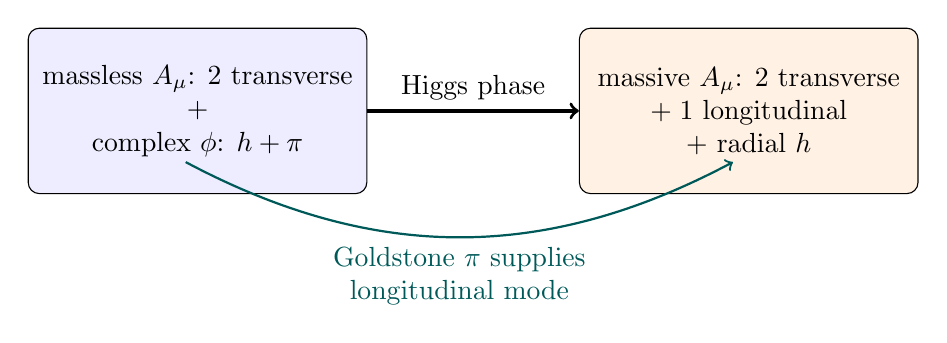
\begin{tikzpicture}[x=1cm,y=1cm]
  \node[draw,rounded corners,fill=blue!7,minimum width=4.3cm,
        minimum height=2.1cm,align=center] (before) at (0,0)
    {massless \(A_\mu\): \(2\) transverse\\
     \(+\)\\
     complex \(\phi\): \(h+\pi\)};
  \node[draw,rounded corners,fill=orange!10,minimum width=4.3cm,
        minimum height=2.1cm,align=center] (after) at (7,0)
    {massive \(A_\mu\): \(2\) transverse\\
     \(+\;1\) longitudinal\\
     \(+\) radial \(h\)};
  \draw[->,very thick] (before) -- node[above]{Higgs phase} (after);
  \draw[->,teal!70!black,thick]
    (-0.15,-0.65) to[bend right=28]
    node[below,align=center]{Goldstone \(\pi\) supplies\\longitudinal mode}
    (6.8,-0.65);
\end{tikzpicture}
\end{adjustbox}
\caption{Механизм Хиггса не уничтожает физические степени свободы, а перераспределяет их.}
\label{fig:l08-degree-rearrangement}
\end{figure}

\begin{classroomqa}
\audiencequestion{Как может угловая степень свободы исчезнуть, не нарушая подсчёта степеней свободы?\lecturetimestamp{01:19:13}}
\lecturerresponse{Физически она не исчезает. Безмассовый вектор имеет две спиральности, потому что его нельзя перевести в состояние покоя. Массивный вектор имеет три поляризации, включая продольную. Голдстоуновская мода становится этой третьей поляризацией, так что общий счёт остаётся прежним.}
\end{classroomqa}

В лекции предлагается полезный кинематический тест. Представьте массивную векторную частицу, замедлите её до состояния покоя, а затем разгоните в новом направлении. Поляризация, которая была поперечной относительно исходного движения, может стать продольной относительно нового движения. Точно так же, если циркулярно поляризованную массивную частицу провести через состояние покоя и направить в противоположную сторону, её метка спиральности меняется на противоположную. Строго безмассовую частицу нельзя провести через такой эксперимент, потому что ни одна инерциальная система отсчёта не может привести её к покою. Поэтому две её спиральности образуют непротиворечивый физический спектр.

\section{Сверхпроводящий аналог}

В обычном сверхпроводнике электроны образуют куперовские пары. Пара — это бозон с электрическим зарядом \(2e\), а конденсат описывается заряженным комплексным параметром порядка. Когда его модуль отличен от нуля, сочетание его фазы с электромагнитным векторным потенциалом порождает механизм Андерсона--Хиггса. Статические магнитные поля затухают на лондоновской глубине проникновения, а не распространяются свободно в толще материала. В этом точном, зависящем от среды смысле фотон ведёт себя так, как если бы он приобрёл массу.

Этот пример также проясняет различие, с которого мы начали. Электромагнитное поле не превращается навсегда в другую элементарную частицу. Характер распространения, соответствующий массивной частице, свойствен коллективному состоянию внутри материала; снаружи вакуумный фотон остаётся безмассовым.

\section{Что было установлено}

Теперь этот аргумент можно сжато изложить, не теряя его логики:
\begin{enumerate}
  \item Нарушенная глобальная непрерывная симметрия имеет плоское угловое направление и потому безмассовую голдстоуновскую моду.
  \item Локальная фазовая инвариантность требует калибровочного потенциала и заменяет \(\partial_\mu\) на \(D_\mu\).
  \item Голый массовый член \(A_\mu A^\mu\) нарушает закон локального преобразования.
  \item Когда заряженный скаляр имеет ненулевой равновесный модуль \(f\), калибровочно-инвариантный член \(|D_\mu\phi|^2\) содержит \(\frac12g^2f^2A_\mu A^\mu\).
  \item Фазу можно устранить выбором калибровки, и её физическая степень свободы становится продольной поляризацией массивного вектора.
  \item Радиальное возбуждение Хиггса остаётся, а его масса определяется кривизной скалярного потенциала.
\end{enumerate}

Следующая задача — дать массы фермионам. Электроны и кварки не могут напрямую использовать векторный механизм; их связи с Хиггсом являются взаимодействиями Юкавы. Когда скалярное поле устанавливается на \(f\), эти взаимодействия становятся массовыми членами фермионов.

Широкое утверждение о том, что без нарушения электрослабой симметрии привычные частицы были бы безмассовыми, требует ещё одного последнего уточнения. Массы элементарных кварков и заряженных лептонов, а также массы \(W\) и \(Z\), действительно обращаются в нуль вместе со средним значением поля Хиггса. Однако большая часть массы протона и нейтрона возникает динамически из конфайнмента КХД и энергии сильного поля, а не из хиггсовских масс кварков. Это различие не меняет выведенный здесь механизм Хиггса; оно лишь точно очерчивает область его применимости.